\chapter{قياس الطول}\label{ch:g2:measuring-length}

بابان في بيتين مختلفين: أيّهما أعلى؟ لا تستطيع أن تحمل بابًا عبر
المدينة لتنصبه إلى جانب الآخر. في السنة الماضية قارنّا الأشياء
جنبًا إلى جنب؛ وهذه السنة نتعلّم أعظم حيلة في العلم --- تحويل
الطول إلى \emph{عدد} يستطيع السفر.

\section{المقارنة بلا أعداد}

\begin{example}[جنبًا إلى جنب]\label{ex:g2:measuring-length:sidebyside}
لتعرف أطول القلمين، انصبهما معًا على الطاولة: الذي يبرز هو الفائز.
ولتقارن طولك بطول صديقك، قِفا ظهرًا إلى ظهر. وهذا يفلح فلاحًا
جميلًا --- ما دام الشيئان يمكن أن يجتمعا.
\end{example}

\begin{example}[حيلة الخيط]\label{ex:g2:measuring-length:string}
البابان لا يستطيعان اللقاء --- لكن الخيط يستطيع زيارتهما معًا. مُدّ
خيطًا على الباب الأول واقطعه عند ذلك الارتفاع بالضبط. ثم احمل
الخيط إلى الباب الثاني: إن قصر الخيط فالباب الثاني أعلى. الخيط
يحمل ارتفاع الباب الأول عبر المدينة. وخطوة أفضل: ماذا لو استطعنا
أن نرسل الارتفاع في \emph{رسالة}؟ لذلك نحتاج إلى الأعداد.
\end{example}

\section{القياس بالخطوات والأشبار}

\begin{definition}[قياس طول]\label{def:g2:measuring-length:measure}
أن \emph{تقيس}\index{قياس} طولًا هو أن تعدّ كم مرة تنطبق عليه
\emph{وحدة}\index{وحدة} مختارة --- خطوة، أو شبر يد، أو عصا صغيرة
--- طرفًا إلى طرف بلا فجوات ولا تداخل. والجواب عدد من الوحدات:
``طول الغرفة $12$ خطوة.''
\end{definition}

\begin{example}[جرّب: اقطع الغرفة بقدميك]\label{ex:g2:measuring-length:pace}
اقطع غرفة نومك واضعًا عقبًا إلى إصبع، وعُدّ أطوال قدمك. واطلب من
شخص كبير أن يفعل مثلك. قد تعدّ أنت $18$ قدمًا ويعدّ الكبير $12$
فقط --- \emph{للغرفة نفسها}! ولم يخطئ أحد في العدّ: قدمك أقصر،
فيدخل منها عدد أكبر. \omterm{def:g2:measuring-length:measure}{والقياس} المصنوع بقدمي \emph{أنا} لا يمكن
التحقّق منه بقدم \emph{أنت}.
\end{example}

\begin{omfigure}
\begin{tikzpicture}[scale=0.8]
  \draw[thick] (0,1.6) -- (9,1.6);
  \foreach \i in {0,...,11} {
    \draw[omDef, thick] (\i*0.75,1.6) rectangle ++(0.75,0.28);
  }
  \node[right, font=\small] at (9.2,1.74) {الطفل: $12$ قدمًا صغيرة};
  \draw[thick] (0,0) -- (9,0);
  \foreach \i in {0,...,7} {
    \draw[omThm, thick] (\i*1.125,0) rectangle ++(1.125,0.28);
  }
  \node[right, font=\small] at (9.2,0.14) {الكبير: $8$ أقدام كبيرة};
\end{tikzpicture}

{\small الجدار نفسه، مقيسًا مرتين: $12$ قدمًا صغيرة، أو $8$ أقدام
كبيرة. أقدام مختلفة وأعداد مختلفة --- والجدار لم يتغيّر.}
\end{omfigure}

\begin{remark}[الخصومة في السوق]\label{rem:g2:measuring-length:argument}
كان الناس زمنًا طويلًا يقيسون فعلًا بالأقدام والأصابع وباع
الذراعين، وكانت الأسواق ترنّ بالخصومات: قدم مَن؟ أقدم التاجر
الطويل أم قدم الزبون القصير؟ وكان الحلّ، وقد اتُّفق عليه في العالم
كله، أن تُختار \omterm{def:g2:measuring-length:measure}{وحدة} \emph{واحدة} للجميع --- \omterm{def:g2:measuring-length:measure}{وحدة} لا تخصّ جسد
أحد.
\end{remark}

\section{السنتيمتر والمتر}

\begin{definition}[السنتيمتر والمتر]\label{def:g2:measuring-length:units}
\emph{السنتيمتر}\index{سنتيمتر} (ويُكتب \unit{cm}) \omterm{def:g2:measuring-length:measure}{وحدة} طول صغيرة،
في عرض الظفر تقريبًا؛ وهو مطبوع على كل مسطرة.
و\emph{المتر}\index{متر} (ويُكتب \unit{m}) \omterm{def:g2:measuring-length:measure}{وحدة} كبيرة، تساوي $100$
سنتيمتر بالضبط، وهي طول خطوة كبيرة جدًّا. وهاتان الوحدتان واحدة
عند كل من على الأرض: فالمقدار \qty{20}{cm} عندك يساوي المقدار
\qty{20}{cm} عندي تمامًا.
\end{definition}

\begin{omfigure}
\begin{tikzpicture}[scale=0.85]
  \draw[thick] (0,0.5) rectangle (10,1.1);
  \foreach \i in {1,...,9} {
    \draw (\i,0.5) -- (\i,0.85);
  }
  \node[below, font=\small] at (0,0.4) {$0$};
  \node[below, font=\small] at (5,0.4) {$50$};
  \node[below, font=\small] at (10,0.4) {$100$};
  \node[above, font=\small] at (5,1.35)
    {$100$ خطوة صغيرة من \unit{cm} تصنع \qty{1}{m}};
\end{tikzpicture}

{\small عصا \omterm{def:g2:measuring-length:units}{المتر}: مئة \omterm{def:g2:measuring-length:units}{سنتيمتر} في صفّ واحد. والعلامات تتيح عدّها
بسرعة بدل عدّها واحدًا واحدًا.}
\end{omfigure}

\begin{method}[القياس بالمسطرة]\label{met:g2:measuring-length:ruler}
\begin{enumerate}
  \item ضع المسطرة على طول الجسم ملامسة له؛
  \item ضع \emph{علامة الصفر} في المسطرة عند أحد طرفَي الجسم
        بالضبط --- لا حافة المسطرة، بل العلامة $0$؛
  \item اقرأ العدد عند الطرف الآخر: ذلك هو الطول
        بالسنتيمترات.
\end{enumerate}
وإن وقع الطرف بين علامتين فقل ``بين \qty{7}{cm} و\qty{8}{cm}،
أقرب إلى $8$'' --- فالكلام الأمين خير من عدد مختلَق.
\end{method}

\begin{omfigure}
\begin{tikzpicture}[scale=0.85]
  \draw[thick] (0,0) rectangle (8.4,0.7);
  \foreach \i in {0,...,12} {
    \draw (0.2+\i*0.65,0) -- (0.2+\i*0.65,0.3);
    \node[below, font=\footnotesize] at (0.2+\i*0.65,0) {\i};
  }
  \draw[thick, fill=omMeth, fill opacity=0.5]
    (0.2,1.0) rectangle (5.4,1.45);
  \node[font=\small] at (2.8,1.22) {قلم تلوين};
  \draw[dashed, omExo] (0.2,0.35) -- (0.2,1.0);
  \draw[dashed, omExo] (5.4,0.35) -- (5.4,1.0);
  \node[above, font=\small] at (5.4,1.5) {نقرأ $8$: \qty{8}{cm}};
\end{tikzpicture}

{\small قراءة المسطرة: علامة الصفر عند أحد طرفَي قلم التلوين، ثم
اقرأ الطرف الآخر. طول هذا القلم \qty{8}{cm}.}
\end{omfigure}

\begin{omfigure}
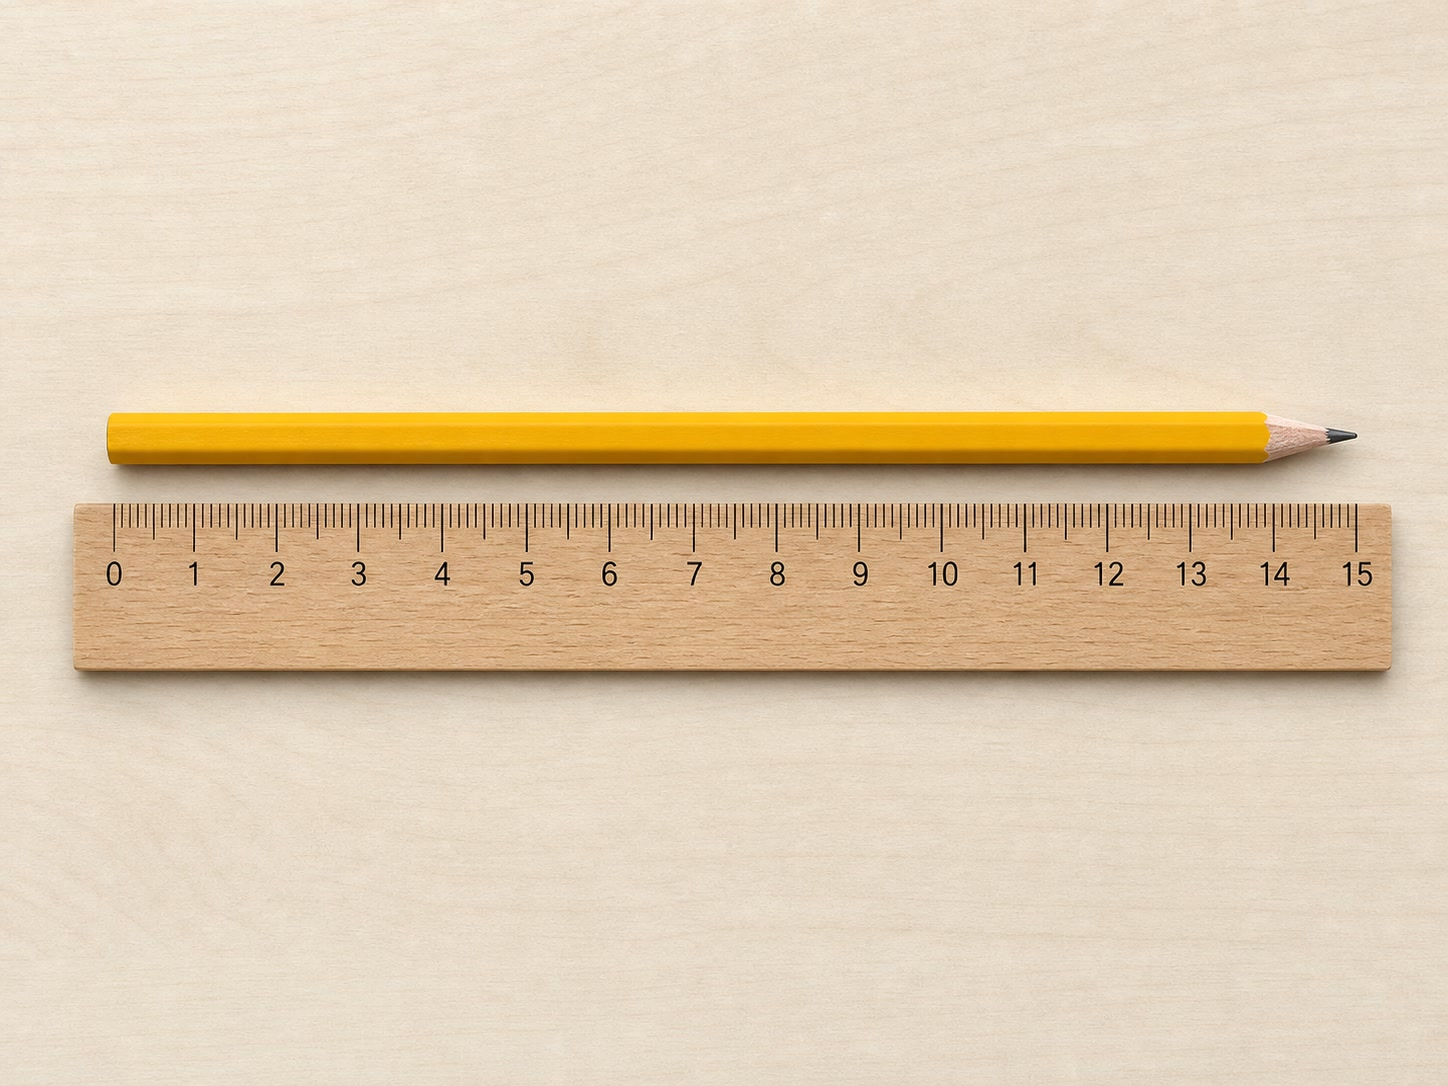
\includegraphics[width=0.52\linewidth]{images/book1/ai/g2-measuring-ruler.jpg}

{\small \omterm{def:g2:measuring-length:measure}{قياس} على أصوله: طرف القلم يقع على علامة الصفر في المسطرة بالضبط.}
\end{omfigure}

\begin{example}[أيّ وحدة لأيّ عمل؟]\label{ex:g2:measuring-length:whichunit}
الأشياء الصغيرة مثل خنفساء أو طابع بريد أو يدك تُقاس
بالسنتيمترات. والأشياء الكبيرة مثل ممرّ أو حافلة أو حوض سباحة
تُقاس بالأمتار: فطول الحوض \qty{25}{m} --- تخيّل عدّ ذلك بعروض
الأظافر! واختيار \omterm{def:g2:measuring-length:measure}{وحدة} معقولة نصف عمل \omterm{def:g2:measuring-length:measure}{القياس}.
\end{example}

\begin{example}[قدّر، ثم تحقّق]\label{ex:g2:measuring-length:estimate}
قبل \omterm{def:g2:measuring-length:measure}{القياس} يتوقّع اللاعبون: كم طول طاولة المطبخ؟ يقول بابا
\qty{2}{m}، وتقول لينا \qty{1}{m} وشيئًا. ثم تفصل عصا \omterm{def:g2:measuring-length:units}{المتر}:
\qty{1}{m} ونصف تقريبًا --- نقطة للينا. التوقّع أولًا يدرّب
عينك؛ \omterm{def:g2:measuring-length:measure}{والقياس} يبقي الجميع أمناء.
\end{example}

\section{تمارين}

\begin{exercise}[$\star$]\label{exo:g2:measuring-length:1}
كيف تقارن طولك بطول صديق من غير أي مسطرة؟ وكيف تقارنه بطول صديق
يسكن مدينة أخرى؟
\end{exercise}

\begin{exercise}[$\star$]\label{exo:g2:measuring-length:2}
\omterm{def:g2:measuring-length:measure}{تقيس} مارا الصفّ بالخطوات فتجد $20$؛ ويجد معلّمها $14$. مَن أخطأ
في العدّ؟ اشرح.
\end{exercise}

\begin{exercise}[$\star$]\label{exo:g2:measuring-length:3}
ما الذي يميّز \omterm{def:g2:measuring-length:units}{السنتيمتر} عن طول القدم أو شبر اليد؟ ولماذا اتّفق
الناس عليه؟
\end{exercise}

\begin{exercise}[$\star$]\label{exo:g2:measuring-length:4}
أيّ \omterm{def:g2:measuring-length:measure}{وحدة} أنسب، \unit{cm} أم \unit{m}: طول نملة؛ \ ارتفاع باب؛
\ طول ساحة المدرسة؛ \ عرض هذا الكتاب؟
\end{exercise}

\begin{exercise}[$\star$]\label{exo:g2:measuring-length:5}
يضع تيم حافة مسطرته --- لا علامة الصفر --- عند طرف قلمه، ويقرأ
\qty{13}{cm}. أطول قلمه \qty{13}{cm} حقًّا؟ وماذا نسي من
\cref{met:g2:measuring-length:ruler}؟
\end{exercise}

\begin{exercise}[$\star$]\label{exo:g2:measuring-length:6}
قِس بالمسطرة: عرض يدك؛ \ طول ملعقة؛ \ ارتفاع كوب. واكتب كل
جواب مع وحدته.
\end{exercise}

\begin{exercise}[$\star$]\label{exo:g2:measuring-length:7}
ارتفاع باب \qty{2}{m}. كم سنتيمترًا يكون ذلك؟ (تذكّر:
\qty{1}{m} تساوي $100$ \unit{cm}.)
\end{exercise}

\begin{exercise}[$\star$]\label{exo:g2:measuring-length:8}
توقّع أولًا، ثم قِس: كم مترًا يبلغ طول سريرك؟ أكان توقّعك أكبر
من الحقيقة أم أصغر أم قريبًا منها؟
\end{exercise}

\begin{exercise}[$\star\star$]\label{exo:g2:measuring-length:9}
شريط طوله \qty{45}{cm}، وآخر طوله \qty{38}{cm}. أيّهما أطول، وبكم
سنتيمترًا؟ أكان يمكن أن تحسم الأمر \emph{بلا} أعداد؟ وأيّ الطريقتين
أسهل كتابةً في رسالة؟
\end{exercise}

\begin{exercise}[$\star\star$]\label{exo:g2:measuring-length:10}
يقول الجدّ: ``طول حديقتي $30$ خطوة.'' اشرح للجدّ برفق لماذا لا
يستطيع غيره أن يتحقّق من ``$30$ خطوة''، وما الذي ينبغي أن يستعمله
بدلًا من ذلك. وماذا يحدث لو قطع طفل صغير الحديقة نفسها بخطواته؟
\end{exercise}
